\documentclass{standalone}
\usepackage{tikz}
\usetikzlibrary{shapes.multipart}
\usepackage{etoolbox}


\tikzset{
  e/.style={draw, -latex, thick},
  w/.style={auto, font=\small, inner sep=2pt},
  layer/.style 2 args={
    rectangle split,
    rectangle split horizontal,
    draw=#2,
    rectangle split parts=#1,
    fill=#2!40,
    outer sep=1pt,
  },
}

\begin{document}

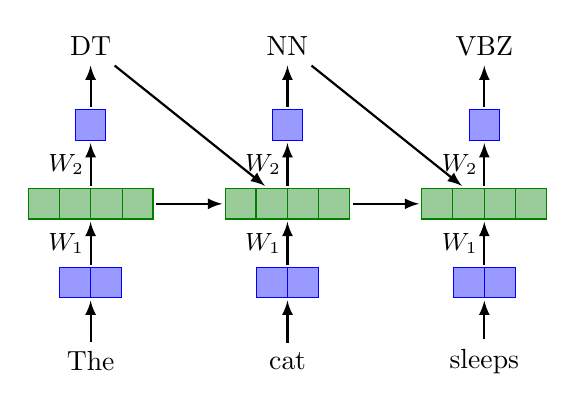
\begin{tikzpicture}
\pgfmathsetmacro{\height}{1}
\pgfmathsetmacro{\width}{2.5}

\foreach \word/\label [count=\i from 0, remember=\i as \lasti] in {The/DT, cat/NN, sleeps/VBZ} {
  \node (label\i) at (\i*\width, 3*\height) {\label};
  \node[layer={1}{blue}] (output\i) at (\i*\width, 2*\height) {} edge[e] (label\i);
  \node[layer={4}{green!50!black}] (hidden\i) at (\i*\width, 1*\height) {} edge[e] node[w] {$W_2$} (output\i);
  \node[layer={2}{blue}] (input\i) at (\i*\width, 0) {} edge[e] node[w] {$W_1$} (hidden\i);
  \node (word\i) at (\i*\width, -1*\height) {\word} edge[e] (input\i);
  \ifdefstring{\i}{0}{}{
    \draw[e] (hidden\lasti) -- (hidden\i);
    \draw[e] (label\lasti) -- (hidden\i);
  }
}

\end{tikzpicture}

\end{document}
